Recall that false sharing is caused when two CPUs what to access two different data in the same cache block because cache coherency prevents two CPUs from reading and wrtting in the the same cache block
, this creates an unessary wast of time since the two data they want to access are not from the same location.
A naive approch to solving this problem is to just get rid of cache coherence,
 but this will cause chaous when multiple processors are tring to read and write to the same data location known as data race. Therefore a good approch in reducing false sharing must not disterbe the perpos on having cache coherency in the fist place.

\section{Reducing False Sharing through Compile Time Data Transformations}

Instaed of altering the cache coherence protocal one way to reduce false sharing is by organizing the data in such a way that false sharing is less liking to occur.
In \citealp{jeremiassen1995reducing} suggest that this may be done by the compiler. Increasing the compilation time, but decreasing the running time.
For false sharing to not occur, data that are access by only one processors must be grouped togather in the same cahce block, and data that is shared by multiple processors with no processor locality do not share cache blocks.
By grouping data that are used by the same processor togather, it ensures that the probability of haveing two processors accessing the same cahce block is reduce greatly, which interns reduces false sharing.
To acomplish this \citealp*{jeremiassen1995reducing} have stated three techniques to reduce false sharing which are group and transpose, indirection, and pad and alingn.

\subsection*{Group and Transpose}
group and transpose works by crated vectors such that adjacent elements in a vector are accessed by different processors and then tranpose it.
If any processor's data is less than the cahce block size then it may be padded.
This is to ensure that no two processors share the same cache block.
Inaddition to reduceing false sharing, This transformation improves spatial locality,
which means that data that is access by the same processor are more liky to be in the same chahe block incresing the retrival time of some data.

\subsection*{Indirection}
When it is not posible to group data togather, we can acomplish something similar by using pointers or indirection. This is done by allocating an array of data areas that is going to be access by a specific prossor,
place shared data into them, and locates the share data with pointers that replace the values of the original data.

\subsection*{Pad and Align}
Another way of reducing false sharing is to use padding. This works by padding data that is going to be access by only one processor so that it completly fills the cache block. This makes it so that no other data can be place in the same cache block.
Although this method does reduce false sharing, it is not space efficient since the padded space can not be use to keep data.
Moreover, by haveing each data in it's own cache block it gradly reduces spatial locality.
In order to use this method effactively, it is best to pad data that are almost as large as the cache block or data that is risk of creating false sharing.


\begin{figure}[h]
        \centering
        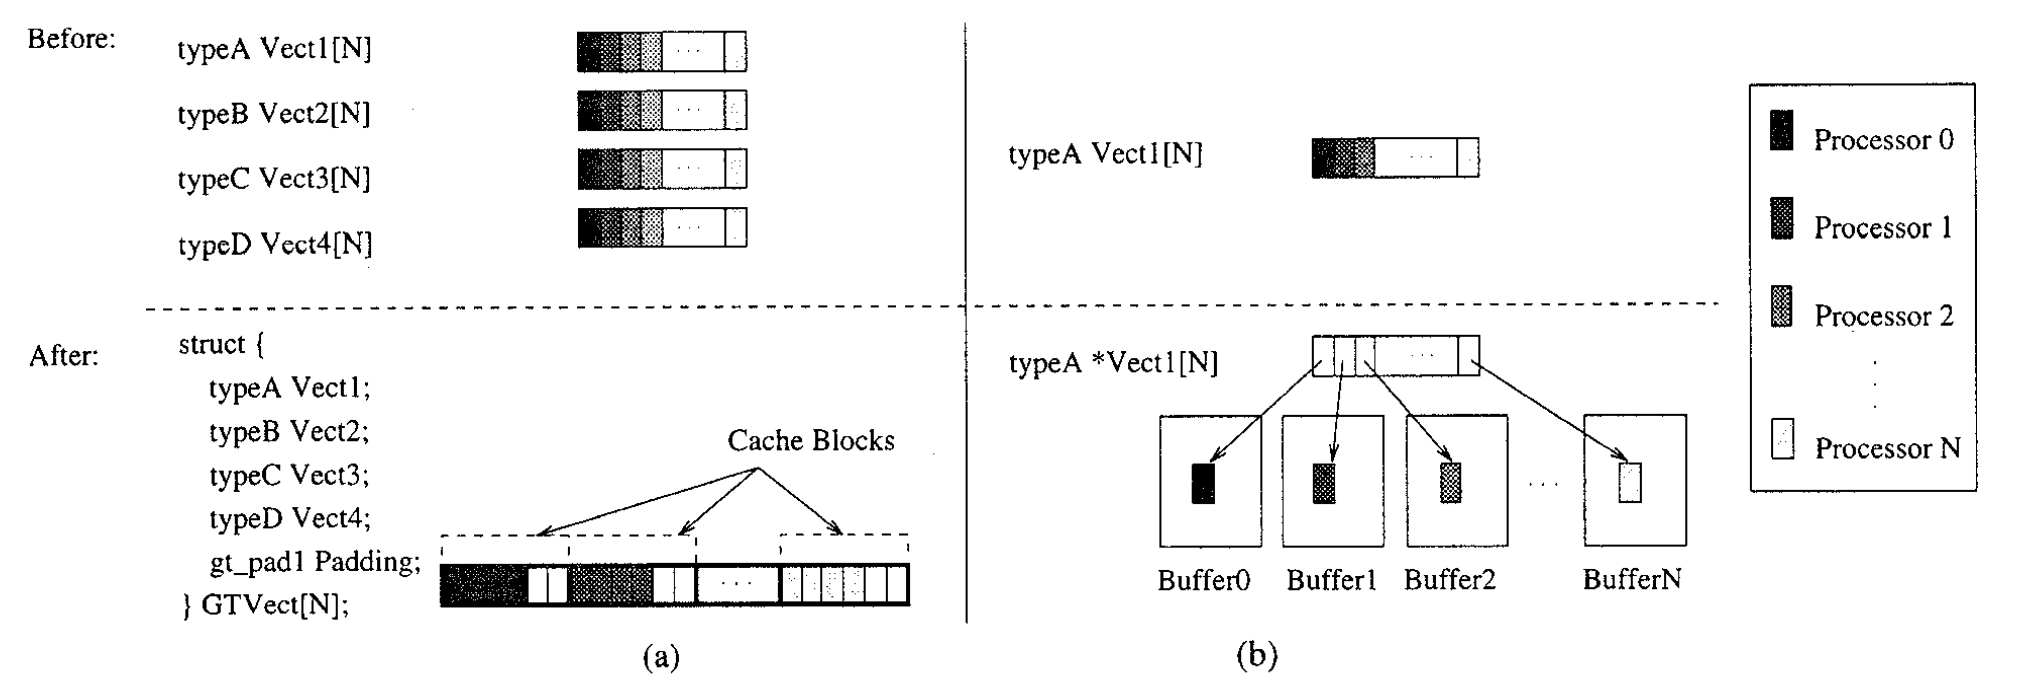
\includegraphics[width=1\textwidth,scale=0.5]{solutions.png}
        \caption{\label{fig:false_sharing_solutions} (a) group and transpose, (b) indirection}
\end{figure}

\subsection{Results}
\citealp*{jeremiassen1995reducing} have gien experimental results for the methods of reduceing false sharing on some known algorithms as in figure \ref*{fig:false_sharing_programs}. and the results are given in figure \ref*{fig:false_sharing_table}. 

    


\begin{figure}[h]
        \centering
        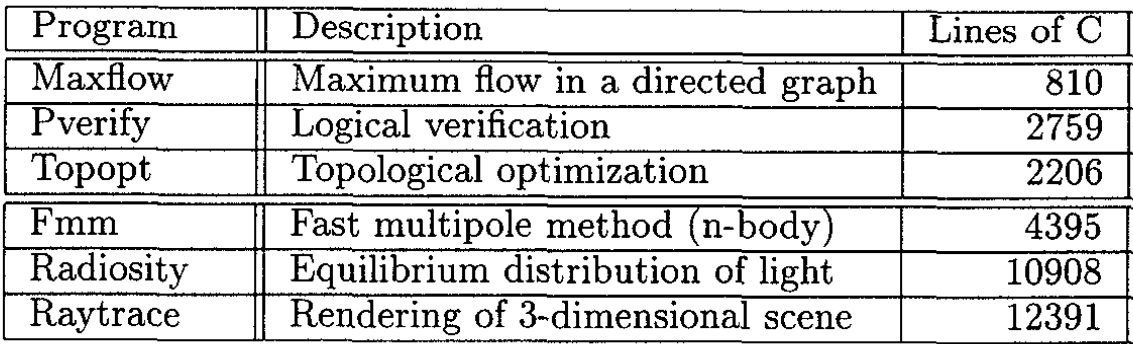
\includegraphics[width=1\textwidth,scale=0.5]{false-sharing_programs.png}
        \caption{\label{fig:false_sharing_programs} Programs that are tested with these methods.}
\end{figure}

\begin{figure}[h]
        \centering
        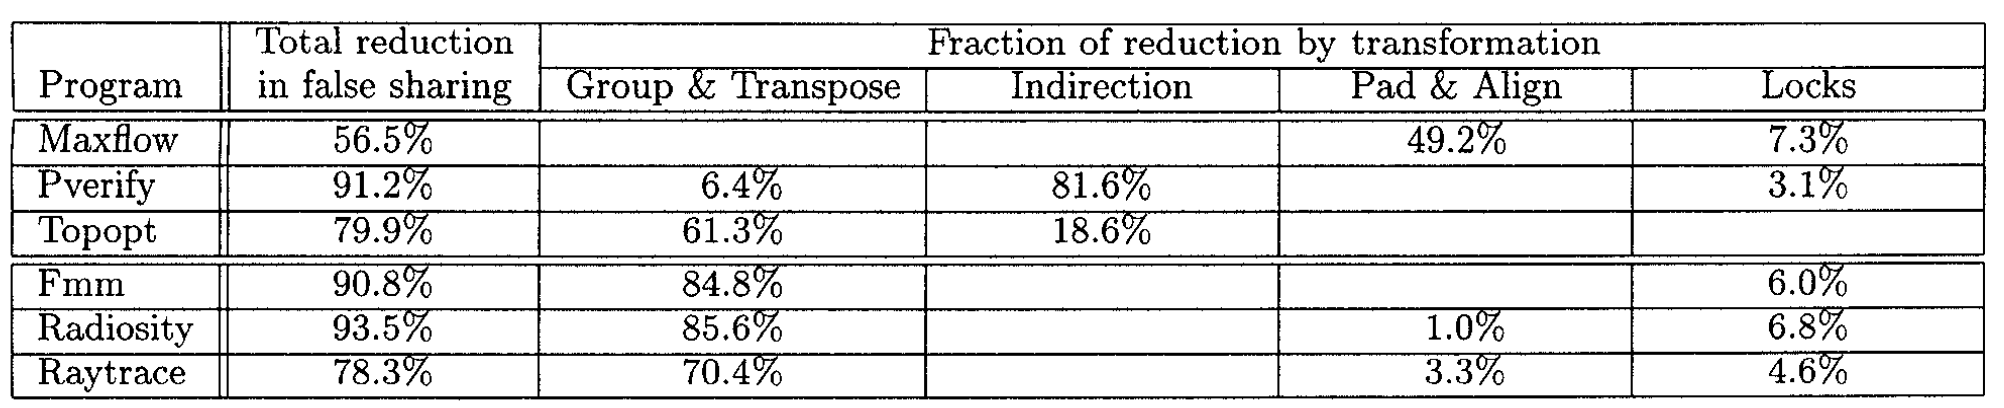
\includegraphics[width=1\textwidth,scale=0.5]{false-sharing_table.png}
        \caption{\label{fig:false_sharing_table} The false sharing miss rate reduction broken down by transformation. Numbers are averages over 8-256 byte cache}
\end{figure}
